\documentclass{beamer}\usepackage[]{graphicx}\usepackage[]{color}
%% maxwidth is the original width if it is less than linewidth
%% otherwise use linewidth (to make sure the graphics do not exceed the margin)
\makeatletter
\def\maxwidth{ %
  \ifdim\Gin@nat@width>\linewidth
    \linewidth
  \else
    \Gin@nat@width
  \fi
}
\makeatother

\definecolor{fgcolor}{rgb}{0.345, 0.345, 0.345}
\newcommand{\hlnum}[1]{\textcolor[rgb]{0.686,0.059,0.569}{#1}}%
\newcommand{\hlstr}[1]{\textcolor[rgb]{0.192,0.494,0.8}{#1}}%
\newcommand{\hlcom}[1]{\textcolor[rgb]{0.678,0.584,0.686}{\textit{#1}}}%
\newcommand{\hlopt}[1]{\textcolor[rgb]{0,0,0}{#1}}%
\newcommand{\hlstd}[1]{\textcolor[rgb]{0.345,0.345,0.345}{#1}}%
\newcommand{\hlkwa}[1]{\textcolor[rgb]{0.161,0.373,0.58}{\textbf{#1}}}%
\newcommand{\hlkwb}[1]{\textcolor[rgb]{0.69,0.353,0.396}{#1}}%
\newcommand{\hlkwc}[1]{\textcolor[rgb]{0.333,0.667,0.333}{#1}}%
\newcommand{\hlkwd}[1]{\textcolor[rgb]{0.737,0.353,0.396}{\textbf{#1}}}%

\usepackage{framed}
\makeatletter
\newenvironment{kframe}{%
 \def\at@end@of@kframe{}%
 \ifinner\ifhmode%
  \def\at@end@of@kframe{\end{minipage}}%
  \begin{minipage}{\columnwidth}%
 \fi\fi%
 \def\FrameCommand##1{\hskip\@totalleftmargin \hskip-\fboxsep
 \colorbox{shadecolor}{##1}\hskip-\fboxsep
     % There is no \\@totalrightmargin, so:
     \hskip-\linewidth \hskip-\@totalleftmargin \hskip\columnwidth}%
 \MakeFramed {\advance\hsize-\width
   \@totalleftmargin\z@ \linewidth\hsize
   \@setminipage}}%
 {\par\unskip\endMakeFramed%
 \at@end@of@kframe}
\makeatother

\definecolor{shadecolor}{rgb}{.97, .97, .97}
\definecolor{messagecolor}{rgb}{0, 0, 0}
\definecolor{warningcolor}{rgb}{1, 0, 1}
\definecolor{errorcolor}{rgb}{1, 0, 0}
\newenvironment{knitrout}{}{} % an empty environment to be redefined in TeX

\usepackage{alltt}
\usetheme{Ilmenau}
\usepackage{amsmath,float,setspace,lmodern,graphicx,
amsthm,amsfonts,multirow,hyperref,bm,bbm,booktabs}

\setbeamertemplate{itemize items}[default]
\setbeamertemplate{enumerate items}[default]

\setbeamercovered{transparent}

\title[Reproducibility with \texttt{git} and \texttt{knitr}]{\texttt{GIT}ting started with reproducibility: \\ An introduction to \texttt{git} and \texttt{knitr}}
\author{Nick Seewald}
\subtitle{Biostatistics Student Association Computing Workshop}
\institute[University of Michigan]{Department of Statistics \\ University of Michigan}
\date{January 29, 2016}
% \logo{\includegraphics[height=.6cm]{blockm.png}}
\IfFileExists{upquote.sty}{\usepackage{upquote}}{}
\begin{document}


	
	\maketitle
	
	\section{Introduction}

	\begin{frame}{Why do I care about reproducibility?}
		Reproducible research is a hallmark of the scientific method, but we're pretty bad at it. 
		
		\begin{quote}
			In 2012, a researcher then at the biotechnology company Amgen wrote in Nature that when his team tried to reproduce 53 landmark cancer studies, they could replicate just six. And according to a news report in Nature, a project aiming to reproduce the findings of 100 psychology papers has managed to replicate results for only 39 of them (the project's findings are still under peer review).
		\end{quote}
		
		\footnotesize{''What Science Can Tell Us About Bad Science'', \textit{The Atlantic}, September 2015.} \scriptsize{\url{http://www.theatlantic.com/magazine/archive/2015/09/a-scientific-look-at-bad-science/399371/}}
	\end{frame}

	\begin{frame}{But I'm a Biostatistician!}
		\begin{itemize}
			\item Reproducibility is important in both science AND statistics!
			\item As statisticians, we need to be able to reproduce our results on the same data set
			\begin{itemize}
				\item This means we have to write reports in a way that minimizes error and write code so that we can get the same results years later.
			\end{itemize}
		\end{itemize}
	\end{frame}
	
	\begin{frame}{Agenda}
		\begin{enumerate}
			\item \texttt{Git}: A ``version control'' tool used for collaborating and maintaining different versions of a file, typically for code.
			\begin{itemize}
				\item Great for collaborating, or just saving your own ass.
				\item Often used in conjunction with \textit{GitHub}, an online repository storage service.
			\end{itemize}
			\item \texttt{knitr}: An R package that lets you create documents containing R code and output.
			\begin{itemize}
				\item Keep everything you need to generate a report (e.g., for research, homework, or 699) in one place!
				\item My favorite part: Update code without having to re-create tables! (This is where errors creep in!)
			\end{itemize}
		\end{enumerate}
	\end{frame}
	
	\section{\texttt{Git}}  
	
	\begin{frame}{A brief warning}

  \begin{figure}
			\centering
			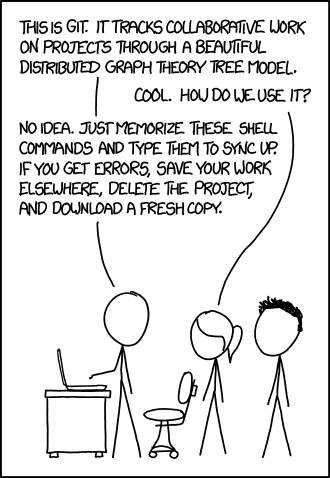
\includegraphics[height=.75\textheight]{xkcd-git.png}
		\end{figure}
		\scriptsize{Source: \url{https://xkcd.com/1597/}}
	\end{frame}
	
	\begin{frame}{Setup}
		Create a GitHub account, then download either Git or GitHub Desktop.
		\begin{itemize}
			\item Pure Git (i.e., just command-line tools): \url{https://git-scm.com/downloads}
			\item GitHub Desktop (GUI \& command-line tools): \url{https://desktop.github.com/}
		\end{itemize}
	\end{frame}
	
	\begin{frame}{Forking a Repository}
		A \textit{fork} is a copy of a repository. Forks let you
		\begin{itemize}
			\item make changes to an existing repo without affecting the original project
			\item use the existing project as a starting point for your own
		\end{itemize}
		One of the benefits of open source!
		
		\textbf{Exercise:} Fork my \texttt{bsa-computing} repository.
	\end{frame}
	
	\begin{frame}{Cloning a Repository}
		\begin{itemize}
			\item To create a local copy of an existing git repository, use 
			\\ \texttt{git clone [url] [directory-name]}.
			\item In a terminal (Mac, Linux) or the Git Shell (Windows), navigate to the folder you want to clone the repository into.
			\item \textbf{Exercise:} Clone your forked \texttt{bsa-computing} repository onto your computer. The URL will be of the form \texttt{https://github.com/[username]/bsa-computing.git}
		\end{itemize}
	\end{frame}
	
	\begin{frame}{Make Changes!}
		\begin{itemize}
			\item You now have a copy of both the current version of \texttt{bsa-computing} \textit{and} access to every previous version.
			\item This clone is NOT automatically synced, \`a la Dropbox
			\begin{itemize}
				\item Anything you break is completely isolated from the pristine copy on GitHub and your previous ``commits''.
			\end{itemize}
			\item \textbf{Exercise:} Add to \texttt{food-exercise.md}, and save your changes.
		\end{itemize}
	\end{frame}
	
	\begin{frame}{Making Commits and Pushing}
		\begin{itemize}
			\item Once you've accomplished a relatively small, but still significant task, you'll want to ``commit'' your code to the repository.
			\item This creates a labeled snapshot of the directory at the time of the commit.
			\item Syncing your commits with the existing remote repository is called ``pushing''.
		\end{itemize}
	\end{frame}
	
	\begin{frame}{Shell Commands for Commits and Push/Pull}
		\begin{itemize}
			\item To \textit{pull} down the most recent version of the remote repository, use \texttt{git pull}
			\item To make and push commits
			\begin{itemize}
				\item Check what you've changed with \texttt{git status} and \texttt{git diff}.
				\item Add files to the commit using \texttt{git add [files]}.
				\item Create a commit using \texttt{git commit -m [message]}
				\item Push your commit to the remote repository using \texttt{git push}
			\end{itemize}
		\end{itemize}
	\end{frame}
	
	\begin{frame}{Merging Your Fork with the Original}
		On GitHub, create a \textit{pull request} to merge your changes into my repository. The owner (me) will be able to look at and accept/decline them.
	\end{frame}
	
	\section{\texttt{knitr}}
	
	\begin{frame}{What is \texttt{knitr}?}
		\begin{itemize}
			\item \texttt{knitr} lets you embed code and output from R into \LaTeX, HTML, RMarkdown, etc. I'll be using \LaTeX.
			\item Might require a bit more thought with R code to get the correct output, but it's worth it.
		\end{itemize}
		The \texttt{knitr} Bible: \url{http://yihui.name/knitr/}
	\end{frame}
	
	\begin{frame}{Chunks}
		\texttt{knitr} separates R code from \LaTeX \ using structures called ``chunks''.
		\begin{block}{Chunk Syntax}
\begin{knitrout}
\definecolor{shadecolor}{rgb}{0.969, 0.969, 0.969}\color{fgcolor}\begin{kframe}
\begin{alltt}
<<\hlkwd{list}\hlstd{(chunkname,} \hlkwc{eval}\hlstd{=}\hlnum{FALSE}>>=
@
\end{alltt}
\end{kframe}


\end{knitrout}
		\end{block}
	\end{frame}
	
		\begin{frame}{Chunk Options}
		When you define a chunk, you also can include a number of options that tell \texttt{knitr} how to interpret the R code inside. Some basic important options are:
		\begin{itemize}
			\item \texttt{echo (TRUE)}: Whether or not to include the R code itself in the document.
			\item \texttt{results}: How to display results. Default is in a \LaTeX \ \texttt{verbatim} environment.
			\begin{itemize}
				\item \texttt{asis}: Write raw results into the document (e.g., with \texttt{xtable})
			\end{itemize}
			\item \texttt{include (TRUE)}: Whether to include the chunk output in the document. The code is still run. Useful for data steps.
			\item \texttt{cache (FALSE)}: Stashes the output of a chunk to avoid running it every time you compile.
		\end{itemize}
		\footnotesize{More options and more details at \url{http://yihui.name/knitr/options/}.}
	\end{frame}
	



	\begin{frame}{Example: Figure}
\begin{knitrout}
\definecolor{shadecolor}{rgb}{0.969, 0.969, 0.969}\color{fgcolor}

{\centering 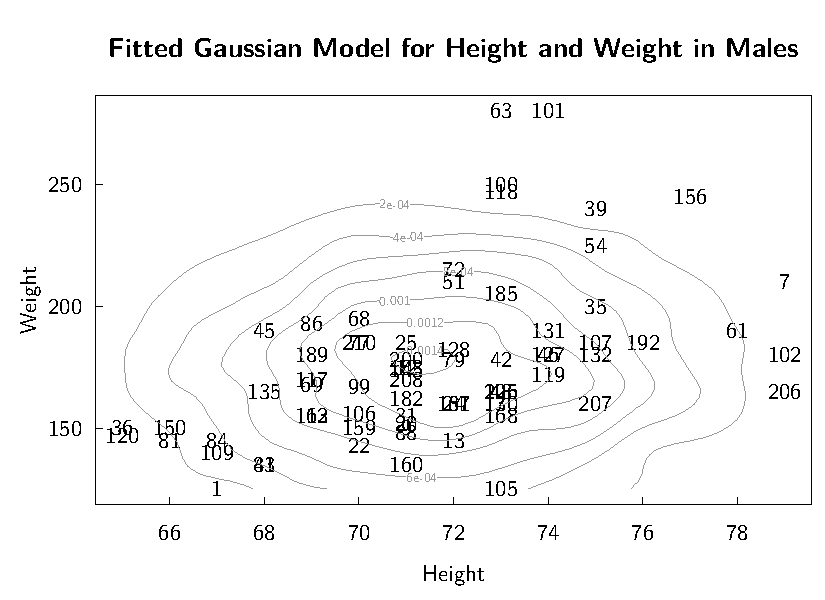
\includegraphics[width=.7\textwidth]{figure/exampleplot-1} 

}



\end{knitrout}
	\end{frame}
	
	\begin{frame}{Example: Tables}
	There are 137 women in this dataset, out of 210 total individuals.
% latex table generated in R 3.2.3 by xtable 1.8-0 package
% Thu Jan 28 23:19:06 2016
\begin{table}[ht]
\centering
\begin{tabular}{rrrr}
  \hline
 & Mean & Std. Dev. & Median \\ 
  \hline
Height & 67.36 & 4.46 & 67.00 \\ 
  Weight & 145.66 & 32.69 & 140.00 \\ 
   \hline
\end{tabular}
\caption{Summary Statistics for All Individuals} 
\end{table}
% latex table generated in R 3.2.3 by xtable 1.8-0 package
% Thu Jan 28 23:19:06 2016
\begin{table}[ht]
\centering
\begin{tabular}{rrrrrrr}
  \hline
 & Min. & 1st Qu. & Median & Mean & 3rd Qu. & Max. \\ 
  \hline
1 & 65.00 & 70.00 & 72.00 & 71.66 & 73.00 & 79.00 \\ 
  2 & 125.00 & 155.00 & 170.00 & 175.60 & 185.00 & 280.00 \\ 
   \hline
\end{tabular}
\caption{Summary Statistics for Men} 
\end{table}

	\end{frame}

\end{document}
